\documentclass[12pt]{article}
\usepackage[utf8]{inputenc}
\usepackage{amsmath}
\usepackage{times}
\usepackage{amsfonts}
\usepackage{amssymb}
\usepackage{graphicx}
\usepackage{tabularx}
\usepackage[font=small,labelfont=bf]{caption}
\usepackage[font=small]{subcaption}
\usepackage{wrapfig}




\begin{document}

\begin{figure}[!htb]
 \centering
 \caption{Wave speed by cross-section of column}
 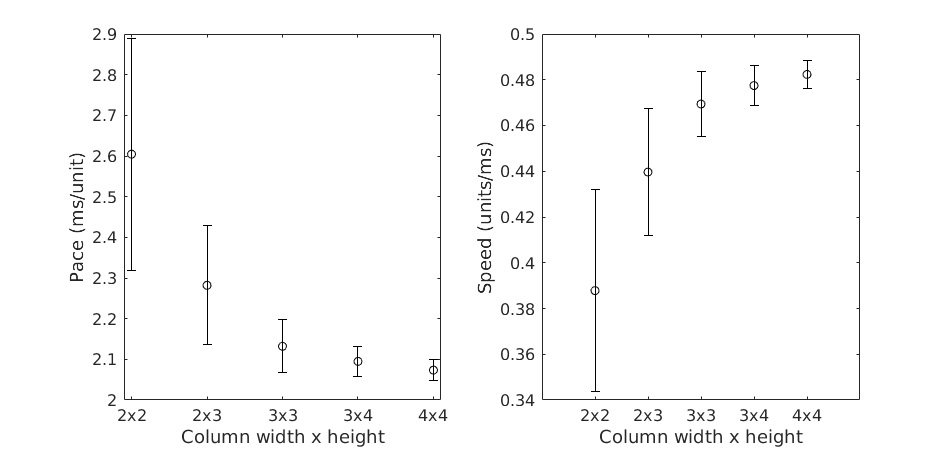
\includegraphics[width=\textwidth]{fig/WaveSpeed_Topology}
\end{figure}



 
\begin{figure}[!htb]
 \begin{tabular}{ccc}
     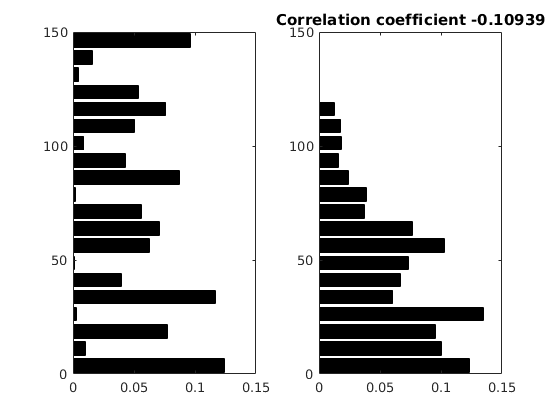
\includegraphics[width=0.3\textwidth]{fig/ccf/ccf1} & 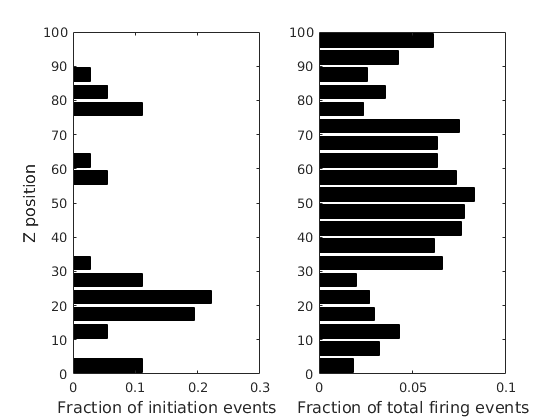
\includegraphics[width=0.3\textwidth]{fig/ccf/ccf2} & 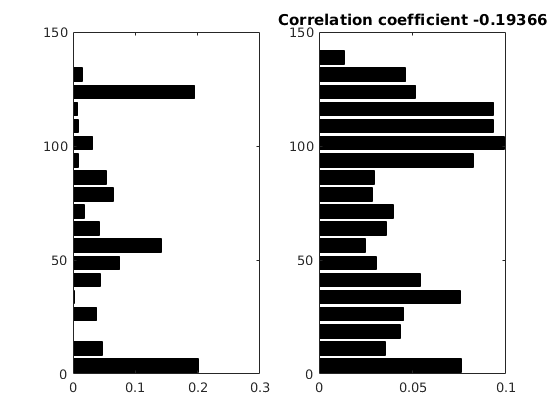
\includegraphics[width=0.3\textwidth]{fig/ccf/ccf3} \\
     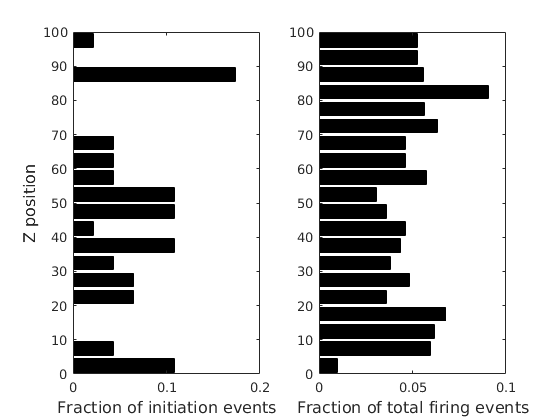
\includegraphics[width=0.3\textwidth]{fig/ccf/ccf4} & 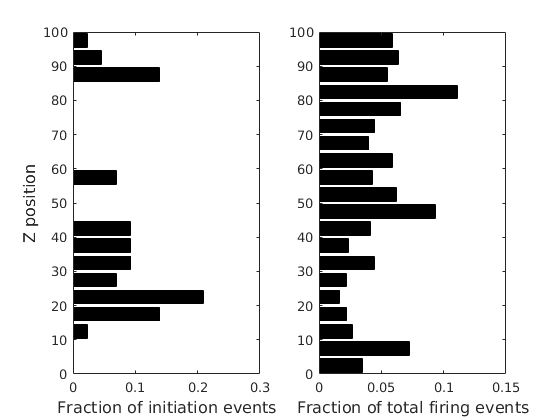
\includegraphics[width=0.3\textwidth]{fig/ccf/ccf5} & 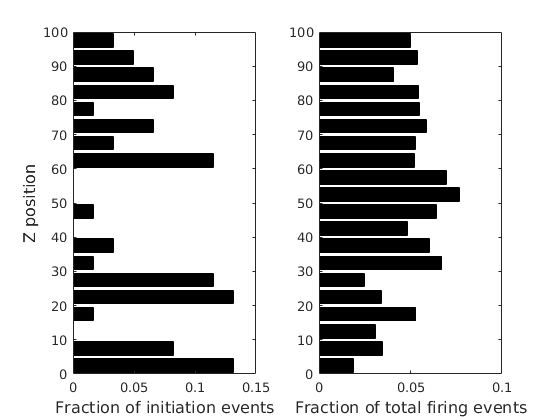
\includegraphics[width=0.3\textwidth]{fig/ccf/ccf6} \\
     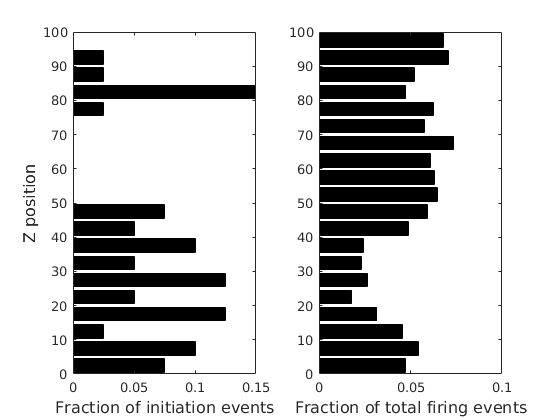
\includegraphics[width=0.3\textwidth]{fig/ccf/ccf7} & 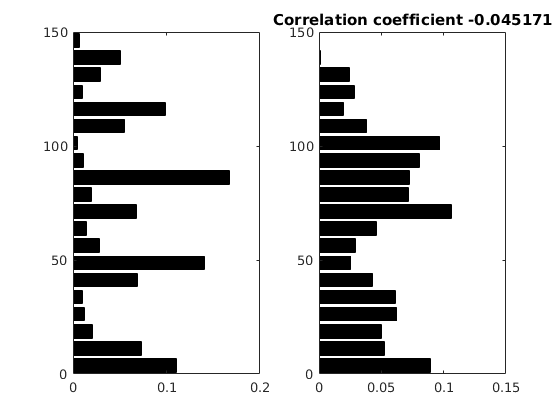
\includegraphics[width=0.3\textwidth]{fig/ccf/ccf8} & 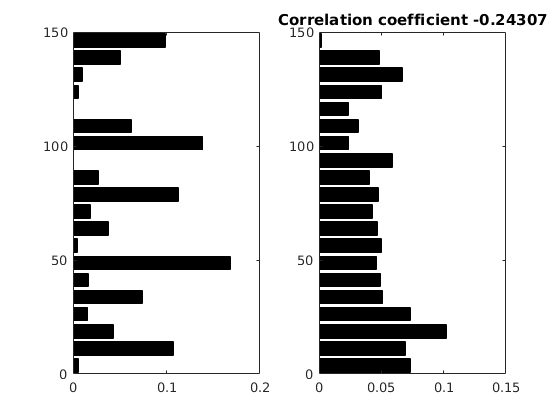
\includegraphics[width=0.3\textwidth]{fig/ccf/ccf9} 
 \end{tabular}
 \caption{FIE and FFE for nine selected columns. }
 
\end{figure}

 
\end{document}
